\documentclass[11pt,a4paper]{article}

\usepackage[T1]{fontenc}
\usepackage{lmodern}
\usepackage[margin=2.5cm]{geometry}
\usepackage{amsmath,amssymb}
\usepackage{booktabs}
\usepackage{tabularx}
\usepackage{enumitem}
\usepackage{xcolor}
\usepackage{tikz}
\usetikzlibrary{arrows.meta,positioning}
\usepackage[hidelinks]{hyperref}
\usepackage[nameinlink]{cleveref}

\setlist{itemsep=2pt,topsep=4pt}

% Notation
\newcommand{\concat}{\mathbin{\|}}
\newcommand{\KDF}{\mathsf{KDF}}
\newcommand{\AEAD}{\mathsf{AEAD}}
\newcommand{\Enc}{\mathsf{Enc}}
\newcommand{\Dec}{\mathsf{Dec}}
\newcommand{\Argon}{\mathsf{Argon2id}}
\newcommand{\Encaps}{\mathsf{Encaps}}
\newcommand{\Decaps}{\mathsf{Decaps}}
\newcommand{\Sign}{\mathsf{Sign}}
\newcommand{\Verify}{\mathsf{Verify}}
\newcommand{\str}[1]{\texttt{"#1"}}
\newcommand{\todo}[1]{\textcolor{red!70!black}{[\textbf{Open:} #1]}}
\newcommand{\dref}[1]{\textsf{#1}} % reference to the decision log in APPDESIGN.md

\title{Cryptographic design of the security core\\[2pt]\large Draft 0.1}
\author{Internal working document}
\date{18 October 2026}

\begin{document}
\maketitle

\begin{abstract}
This document specifies the cryptography of the app's security core (the Rust crate \texttt{secure\_core}): goals, threat model, primitives and cipher suites, the key hierarchy, data at rest, synchronisation, device pairing and sharing. It turns the decisions and proposals of the project's decision log (\texttt{APPDESIGN.md}; identifiers such as \dref{D9} or \dref{P43}) into a precise design that can be reviewed, formally analysed and implemented. Everything not yet decided is marked \todo{like this}. The app's name is deliberately absent; it lives only in the app's \texttt{branding.json} (\dref{D35}).
\end{abstract}

\tableofcontents

\section{Scope and principles}

\begin{itemize}
  \item \textbf{Local-first, no server of ours} (\dref{D4}, \dref{D24}). Data is created, stored and analysed on the user's devices. It moves only directly between devices (peer-to-peer, files) or through storage the user controls (their own cloud storage or server, \dref{D15}). We never receive user data, not even encrypted.
  \item \textbf{Everything at rest and in transit is encrypted}, under keys that only the user's devices hold, protected by a passphrase set during the app's setup (\dref{D9}, \dref{D37}).
  \item \textbf{Quantum-safe} (\dref{D23}): symmetric primitives with 256-bit keys; public-key operations hybrid (classical and post-quantum) unless a scheme from the literature is required (\dref{D25}).
  \item \textbf{Crypto agility} (\dref{D25}, \dref{P46}): every ciphertext, key and signature names its cipher suite and format version, so algorithms can be replaced.
  \item \textbf{A small, separate core} (\dref{D26}): only the core sees keys; the user interface sees decrypted records for display, never key material.
  \item \textbf{Signal as the role model} (\dref{D28}, \dref{P47}): written specification, formal analysis, verified primitives where available, audits, reproducible builds.
\end{itemize}

\section{Security goals}

\begin{enumerate}[label=G\arabic*]
  \item \textbf{Confidentiality} of all user data (training logs, health and body data, photos, videos, notes, the profile) against anyone without the user's keys, including the user's storage provider and network attackers, now and against a future quantum computer (``harvest now, decrypt later'').
  \item \textbf{Integrity and authenticity}: undetected modification, reordering, truncation or forgery of records, sync batches and shares must be impossible.
  \item \textbf{Rollback detection}: a storage provider that serves old data must be detected by devices that have seen newer data.
  \item \textbf{Least disclosure in sharing}: a share reveals only the selected records and fields (\dref{D16}); write access is limited to what the owner granted (\dref{D18}).
  \item \textbf{Recoverability by the user alone}: with the passphrase or the recovery key, and nothing from us.
  \item \textbf{Metadata minimisation}: storage providers learn as little as possible (sizes, counts, timing), see \cref{sec:metadata}.
\end{enumerate}

\noindent\textbf{Non-goals.} Protection against malware with full control of an unlocked device; recovering data when both the passphrase and the recovery key are lost; hiding \emph{that} someone uses the app.

\section{Threat model}

\begin{tabularx}{\textwidth}{@{}lX@{}}
\toprule
Adversary & Capabilities and what the design must achieve \\
\midrule
Thief of a locked device & Has the device's storage. Must not get data without the device unlock (OS keystore) or the passphrase; offline guessing is slowed by Argon2id (\cref{sec:keys}). \\
Storage provider & The user's cloud or server (\dref{D15}): reads, deletes, reorders or replays files, serves old versions. Gets only ciphertext; forgery and rollback are detected (G2, G3). \\
Network attacker & Reads and changes traffic during sync and pairing. Must learn nothing and be unable to impersonate a device. \\
Share recipient & Gets what was shared, and may try to escalate (read more, write without permission) or to impersonate the owner. \\
Compromised web origin & Could serve a malicious browser client (\cref{sec:web}). Mitigated, not eliminated. \\
Future quantum adversary & Breaks discrete logarithms and factoring later, applied to traffic and files recorded today. \\
\bottomrule
\end{tabularx}

\section{Primitives and cipher suites}
\label{sec:suites}

\begin{tabularx}{\textwidth}{@{}lXl@{}}
\toprule
Purpose & Suite 1 (proposal, \dref{P43}, \dref{P46}) & Library \\
\midrule
Authenticated encryption & XChaCha20-Poly1305 (256-bit key, 192-bit random nonce) & libsodium \\
Large files & XChaCha20-Poly1305 per chunk, see \cref{sec:blobs} & libsodium \\
Hash, KDF & BLAKE2b (keyed, with context strings) or HKDF-SHA-256 \todo{choose} & libsodium \\
Passphrase hashing & Argon2id, parameters per platform \todo{benchmark} & libsodium \\
Key encapsulation & X-Wing (X25519 + ML-KEM-768) & libsodium 1.0.22 \\
Signatures & Ed25519 \emph{and} ML-DSA-65; both must verify & libsodium, libcrux \\
Randomness & The operating system's CSPRNG & libsodium \\
\bottomrule
\end{tabularx}

\medskip
\noindent\textbf{Suite identifiers.} Every encrypted object starts with a header $h = (\mathit{format\_version}, \mathit{suite\_id}, \ldots)$ that is bound as associated data, so it can't be changed without detection.

\noindent\textbf{Agility rules} (\dref{P46}):
\begin{itemize}
  \item A registry in the core lists the suites with their status: \emph{active}, \emph{decrypt-only} (broken, being migrated) or \emph{experimental}.
  \item Devices and share partners announce their supported suites in signed form and never accept a suite below a minimum (downgrade protection).
  \item Keys are layered (\cref{sec:keys}), so replacing an algorithm re-wraps keys first and re-encrypts data in the background.
  \item Schemes taken from the research literature (\dref{D25}), e.g.\ threshold schemes, may form the classical or the post-quantum part of a suite. Where the functionality allows, they are combined with an independent, well-studied scheme; otherwise they stand alone and stay \emph{experimental} until reviewed.
\end{itemize}

\section{Key hierarchy}
\label{sec:keys}

\begin{figure}[!ht]
\centering
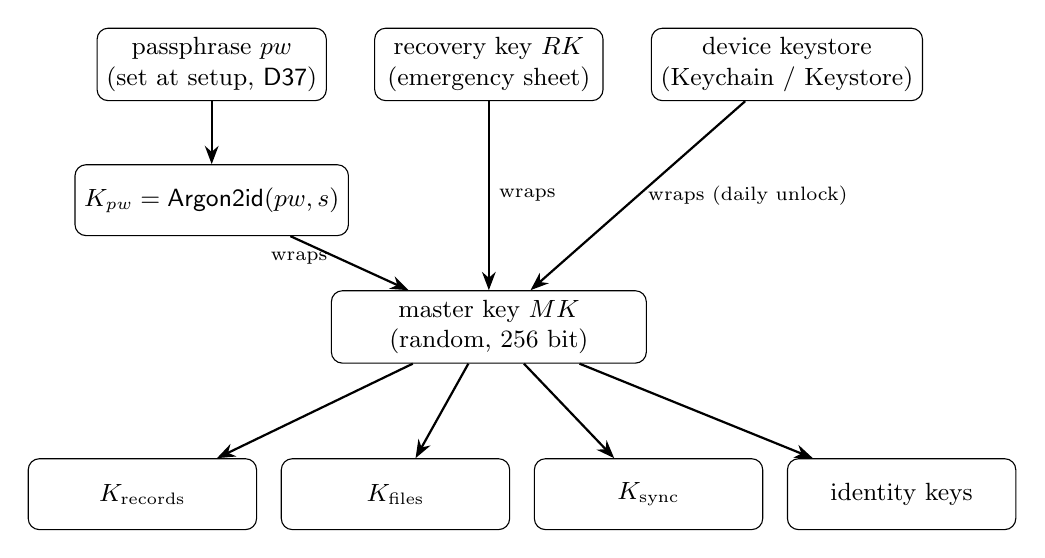
\begin{tikzpicture}[
  box/.style={draw, rounded corners, align=center, minimum width=2.9cm, minimum height=0.9cm, font=\small},
  arr/.style={-{Stealth}, thick}]
  \node[box] (pw) {passphrase $pw$\\(set at setup, \dref{D37})};
  \node[box, right=0.6cm of pw] (rk) {recovery key $RK$\\(emergency sheet)};
  \node[box, right=0.6cm of rk] (dk) {device keystore\\(Keychain / Keystore)};
  \node[box, below=0.8cm of pw] (kpw) {$K_{pw} = \Argon(pw, s)$};
  \node[box, below=2.4cm of rk, minimum width=4cm] (mk) {master key $MK$\\(random, 256 bit)};
  \node[box, below=1.2cm of mk, xshift=-4.4cm] (krec) {$K_{\mathrm{records}}$};
  \node[box, right=0.3cm of krec] (kblob) {$K_{\mathrm{files}}$};
  \node[box, right=0.3cm of kblob] (ksync) {$K_{\mathrm{sync}}$};
  \node[box, right=0.3cm of ksync] (kid) {identity keys};
  \draw[arr] (pw) -- (kpw);
  \draw[arr] (kpw) -- node[left, font=\scriptsize, pos=0.4]{wraps} (mk);
  \draw[arr] (rk) -- node[right, font=\scriptsize]{wraps} (mk);
  \draw[arr] (dk) -- node[right, font=\scriptsize]{wraps (daily unlock)} (mk);
  \draw[arr] (mk) -- (krec);
  \draw[arr] (mk) -- (kblob);
  \draw[arr] (mk) -- (ksync);
  \draw[arr] (mk) -- (kid);
\end{tikzpicture}
\caption{Key hierarchy (proposal). Arrows into $MK$ are key wrapping; arrows out of $MK$ are key derivation.}
\end{figure}

\begin{enumerate}
  \item \textbf{Setup} (\dref{D37}): the app generates $MK \leftarrow \{0,1\}^{256}$, asks for the passphrase $pw$ (with a strength meter and a generated suggestion, \dref{P18}) and generates the recovery key $RK \leftarrow \{0,1\}^{256}$, shown once and on the emergency sheet (\dref{P48}).
  \item \textbf{Passphrase wrap}: $K_{pw} = \Argon(pw, s; t, m, p)$ with a random 128-bit salt $s$; $W_{pw} = \AEAD.\Enc(K_{pw}, n, MK, h)$.
  \item \textbf{Recovery wrap}: $W_{rk} = \AEAD.\Enc(\KDF(RK, \str{recovery}), n, MK, h)$.
  \item \textbf{Device wrap}: a non-exportable key in the OS keystore, unlocked by face, fingerprint or PIN (\dref{P9}), wraps $MK$ for daily use. \todo{exact platform APIs; Secure Enclave on iOS}
  \item \textbf{Optional secret key} (\dref{P18}): a 256-bit device-held secret mixed into $K_{pw}$ so that a stolen backup can't be attacked with the passphrase alone. \todo{decide}
  \item \textbf{Derived keys}: $K_x = \KDF(MK, \str{x} \concat \mathit{suite\_id})$ for $x \in \{$records, files, sync$\}$; identity key pairs are generated randomly and stored encrypted under $MK$.
  \item \textbf{Changes}: changing the passphrase re-wraps $MK$ only. Rotating $MK$ (e.g.\ after losing a device) re-encrypts all data lazily and removes the old device from the device list.
\end{enumerate}

\noindent\textbf{Key handling}: keys exist only inside the core, in memory that is locked where possible and wiped after use (\texttt{zeroize}, \texttt{sodium\_memzero}); the user interface receives opaque handles.

\section{Data at rest}
\label{sec:rest}

\subsection{Records}
Each record $r$ (set, session, meal, measurement, \ldots) has a random identifier $\mathit{rid}$, a type and a version:
\[
c_r = \AEAD.\Enc\big(K_{\mathrm{records}},\ n \leftarrow \{0,1\}^{192},\ \mathrm{encode}(r),\ h \concat \mathit{type} \concat \mathit{rid} \concat \mathit{version}\big).
\]
Binding identifier, type and version as associated data prevents swapping or replaying records under another identity. \todo{storage engine: per-record AEAD in plain SQLite versus SQLCipher pages, and how local queries and analysis work on encrypted data}

\subsection{App settings}
App settings (units, language, theme, timer defaults and alarms, enabled areas) describe how the app behaves, not the athlete. They are stored unencrypted on the device (\dref{D39}), which also lets the app show the right language before it is unlocked. When synced they travel inside the encrypted sync batches like any record (\dref{P58}). Anything that describes the person (profile, weight class, sports) is a record and encrypted.

\subsection{Large files: photos and videos}
\label{sec:blobs}
A random file key $K_f$, wrapped under $K_{\mathrm{files}}$, encrypts the file in chunks of fixed size (e.g.\ 64\,KiB). Chunk $i$ is encrypted with associated data $h \concat \mathit{fid} \concat i \concat \mathit{is\_last}$, so chunks can be decrypted individually (seeking in videos, \dref{P34}) while reordering and truncation are detected. Location metadata is removed before encryption.

\section{Synchronisation}
\label{sec:sync}

\begin{itemize}
  \item \textbf{Operations}: field-level last-writer-wins with hybrid logical clocks (\dref{P22}--\dref{P25}); deletions are tombstones.
  \item \textbf{Batches}: a device groups operations into batches with a header (suite, device identifier, per-device sequence number, clock range). The batch is encrypted under $K_{\mathrm{sync}}$ with the header as associated data and signed with the device's identity key (Ed25519 and ML-DSA-65).
  \item \textbf{Transport-agnostic}: the same encrypted batches move through peer-to-peer connections, files or the user's cloud storage, where each device writes only its own files.
  \item \textbf{Rollback and gaps}: per-device sequence numbers and signed checkpoints of the latest sequence numbers seen let devices detect missing or rolled-back batches. Withholding can be detected, not prevented.
  \item \textbf{Lost device}: another device signs a new device list without it and rotates $MK$ (\cref{sec:keys}).
\end{itemize}

\section{Adding a device}
\label{sec:pairing}

\begin{enumerate}
  \item The existing device shows a QR code with a 256-bit pairing secret $\sigma$ and connection hints.
  \item The new device scans it. Both run a key exchange in which the new device sends an X-Wing public key, the existing device encapsulates to it, and both derive $K_{\mathrm{pair}} = \KDF(ss \concat \sigma, \mathit{transcript})$. Key confirmation in both directions follows.
  \item The existing device sends $MK$ and the device list, encrypted under $K_{\mathrm{pair}}$; the new device adds its identity key, signed by the existing device.
\end{enumerate}
Because $\sigma$ is a symmetric secret, an attacker who later breaks X25519 still lacks $\sigma$; the X-Wing exchange adds forward secrecy. In the browser, this runs inside the WebRTC data channel, whose own encryption isn't quantum-safe. \todo{base it on a Noise pattern with a pre-shared key and a KEM; formal analysis in ProVerif or Tamarin}

\section{Sharing}
\label{sec:sharing}

\begin{itemize}
  \item \textbf{Share container}: each share has a random key $K_{\mathrm{share}}$ and contains only the selected records and fields (\dref{P27}).
  \item \textbf{Key delivery}: for each recipient with an X-Wing public key $pk_R$: $(ct, ss) = \mathsf{XWing}.\Encaps(pk_R)$ and $K_{\mathrm{share}}$ is wrapped under $\KDF(ss, \mathit{share\_id} \concat \mathit{sender\_key\_id} \concat \mathit{recipient\_key\_id})$, in the style of HPKE.
  \item \textbf{Manifest}: share identifier, selection, permissions (read or read-write, \dref{D18}), expiry and recipients, signed by the sender (Ed25519 and ML-DSA-65).
  \item \textbf{Read-write}: a recipient's changes are signed with their identity key; the owner's devices merge them only if the manifest allows those record types and fields.
  \item \textbf{Revocation}: a new $K_{\mathrm{share}}$ for the remaining recipients; revoked recipients keep what they already received.
  \item \textbf{Links for people without the app}: a random key in the URL fragment (never sent to any server), the ciphertext in the sender's own cloud storage (\dref{D24}).
\end{itemize}

\section{The browser client}
\label{sec:web}
The core runs as WebAssembly. Keys live only in memory for the session; a persistent browser copy is treated as a cache (\dref{P38}). Risks: the origin can serve modified code. Mitigations: versioned releases with published hashes, Subresource Integrity, a strict Content Security Policy, an installable app. \todo{WebAuthn PRF (passkeys) as a browser unlock factor where supported}

\section{Metadata}
\label{sec:metadata}
Storage providers see the number, sizes and timing of encrypted files. Mitigations: random file names, padding of records and batches to size buckets, batching of writes. \todo{choose bucket sizes; measure the overhead}

\section{Implementation and assurance}

\begin{itemize}
  \item \textbf{Vetted libraries} behind the suite registry: libsodium 1.0.22 (X-Wing, ML-KEM, XChaCha20-Poly1305, Argon2id, Ed25519); libcrux for ML-DSA (formally verified with hax and F*).
  \item \textbf{Tests} (\texttt{CLAUDE.md}): official test vectors (NIST ACVP, Wycheproof) and our own known-answer tests for every format; a regression test for every fixed bug; fuzzing of all parsers (\texttt{cargo-fuzz}); Miri for any \texttt{unsafe} code; valgrind-based constant-time checks (e.g.\ ctgrind-style) and sanitizers.
  \item \textbf{Formal analysis} of pairing, sync and sharing (ProVerif or Tamarin) before launch; machine-checked implementations where feasible.
  \item \textbf{Independent audit} of the core, reproducible builds, a public vulnerability-reporting policy.
\end{itemize}

\section{Open questions}

\begin{enumerate}
  \item Storage engine and how local analysis works on encrypted records (\cref{sec:rest}).
  \item Argon2id parameters per platform, including phones and browsers with memory limits.
  \item Encoding of the recovery key (word list or groups of characters).
  \item The optional secret key (\dref{P18}).
  \item How often to sign sync batches, given ML-DSA-65's 3{,}309-byte signatures.
  \item Groups and teams later: MLS with post-quantum cipher suites.
  \item Threshold recovery through trusted people, e.g.\ Shamir secret sharing (\dref{D25}).
\end{enumerate}

\begin{thebibliography}{99}
\bibitem{fips203} NIST. \emph{FIPS 203: Module-Lattice-Based Key-Encapsulation Mechanism Standard}. 2024.
\bibitem{fips204} NIST. \emph{FIPS 204: Module-Lattice-Based Digital Signature Standard}. 2024.
\bibitem{xwing} M.~Barbosa, D.~Connolly, J.~Duarte, A.~Kaiser, P.~Schwabe, K.~Varner, B.~Westerbaan. \emph{X-Wing: The Hybrid KEM You've Been Looking For}. IACR ePrint 2024/039; IETF draft draft-connolly-cfrg-xwing-kem.
\bibitem{rfc8439} Y.~Nir, A.~Langley. \emph{ChaCha20 and Poly1305 for IETF Protocols}. RFC 8439, 2018.
\bibitem{rfc9106} A.~Biryukov et al. \emph{Argon2 Memory-Hard Function for Password Hashing and Proof-of-Work Applications}. RFC 9106, 2021.
\bibitem{rfc9180} R.~Barnes et al. \emph{Hybrid Public Key Encryption}. RFC 9180, 2022.
\bibitem{rfc8032} S.~Josefsson, I.~Liusvaara. \emph{Edwards-Curve Digital Signature Algorithm (EdDSA)}. RFC 8032, 2017.
\bibitem{rfc9591} D.~Connolly et al. \emph{The Flexible Round-Optimized Schnorr Threshold (FROST) Protocol}. RFC 9591, 2024.
\bibitem{noise} T.~Perrin. \emph{The Noise Protocol Framework}. Revision 34, 2018.
\bibitem{spqr} Signal. \emph{Signal Protocol and Post-Quantum Ratchets}. Blog post, October 2025.
\bibitem{bsi} BSI. \emph{TR-02102-1: Cryptographic Mechanisms: Recommendations and Key Lengths}. Version 2026-01.
\bibitem{libsodium} F.~Denis. \emph{libsodium documentation}. \url{https://doc.libsodium.org}.
\end{thebibliography}

\end{document}
